\subsection{Architecture}\label{sub:architecture}
ECDAR consists of four major parts as seen in \autoref{fig:ECDAR-architecture}.
There are the two engines, Reveaal and j-Ecdar, as well as the ECDAR GUI, and a test framework as seen in \autoref{fig:ECDAR-architecture}. 
The GUI and the engines communicate through Protocol Buffers (Protobuf) and gRPC (\textbf{G}oogle \textbf{R}emote \textbf{P}rocedure \textbf{C}all) indicated by the arrows.
\begin{figure}[H]
    \centering
    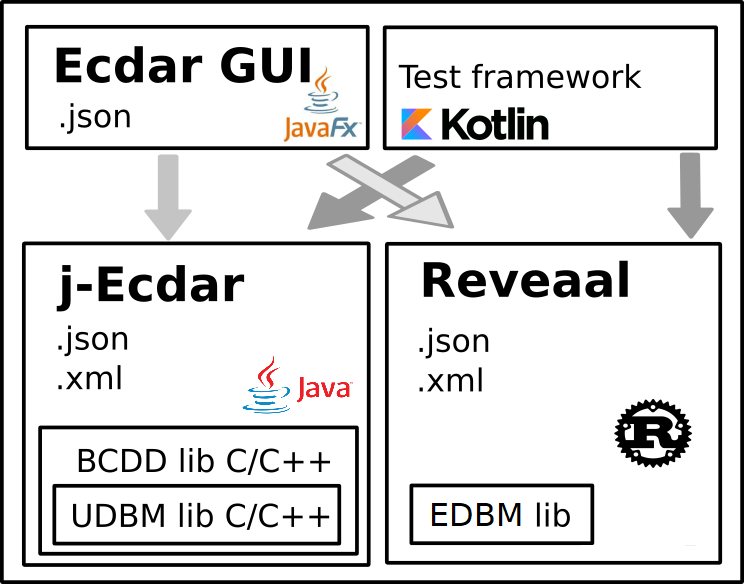
\includegraphics[width=0.75\textwidth]{common/figures/ArchOverview.png}
    \caption{The architecture of ECDAR visualized \cite{ECDARNET}.}
    \label{fig:ECDAR-architecture}
\end{figure}

The graphical user interface (\textbf{GUI}) is written in JavaFX \cite{ECDARNET} which is a graphics and media library for Java. 
The interface provides the tools which enables the user to model their real time systems. 
The GUI sends queries to the engines through gRPC using Protobuf. 
The gRPC and Protobuf frameworks have the advantage of being cross platform and work across languages \cite{gRPC}\cite{google_protocol_nodate}, simplifying the integration process and making it easy to use.

ECDAR runs on two verification engines: j-Ecdar and Reveaal. 
The purpose of having two different engines is to make the whole platform more reliable. 
With two engines, their results can be compared which will help ensure correctness in both engines.
j-Ecdar is an engine written in Java.
The main priorities for this engine are readability and correctness, and, as stated on ECDAR's homepage: ``no effort is put into optimizing the code for speed" \cite{ECDARNET}.
It should be noted here that j-Ecdar will not be worked on this year, as all focus is allotted to the Reveaal engine.
In contrast to j-Ecdar, the Reveaal engine is intended to be fast and parallelizable. 
Recently, the libraries which the engine uses have been rewritten in Rust from C/C++, with the intention of implementing multithreading. 

ECDAR makes use of a testing framework written in Kotlin. 
The testing framework uses a collection of test cases to test both of the engines. 
The testing framework is vital to perform conformance testing between j-Ecdar and Reveaal as well as automated performance testing and hand-designed test cases. 


\subsubsection{gRPC Protocol} \label{subsub:grpc-protocol}
As briefly mentioned previously, the gRPC protocol allows ECDAR to communicate with the two engines.

gRPC is a framework that specifically works for polyglot programs, meaning programs written in multiple languages.
gRPC is used to define a service to tell what methods a client application has access to in a server application.
It means that a client application can directly call a method on a server application, as if it was its own method.
Services specifies methods with a methods parameters and return type.

gRPC uses protocol buffers, which will now be referred to as ProtoBuf, to serialize structured data send between a client application and server application.
The data in ProtoBuf are structured in \textit{messages} which contains a series of name-value pairs.

In ECDAR, gRPC is responsible for sending queries and models from the GUI to one of the engines where the engines then sends the results back via gRPC.
